\section{Replicator suppressor}



\definecolor{Rec}{HTML}{008000}
\definecolor{Rup}{HTML}{992600}
\definecolor{gray1}{HTML}{d9d9d9}%{cccccc}
\definecolor{na1}{HTML}{4d94ff}
\definecolor{nb1}{HTML}{d6b129}
\definecolor{mut1}{HTML}{80d5d5}
\definecolor{Rec2}{HTML}{40bf40}
\definecolor{Rup2}{HTML}{c67053}
\definecolor{blu}{HTML}{002266}



% Define custom colors that match the colors in the provided image
\definecolor{spyder5keyword}{rgb}{0.15, 0.15, 0.7}   % Orange for keywords
\definecolor{spyder5comment}{rgb}{0.25, 0.50, 0.37}  % Greenish for comments
\definecolor{spyder5string}{rgb}{0.56, 0.0, 0.56}    % Purple for strings
\definecolor{spyder5number}{rgb}{0.19, 0.55, 0.91}   % Light blue for numbers
\definecolor{spyder5identifier}{rgb}{0.81, 0.85, 0.87} % Light gray for identifiers
\definecolor{spyder5background}{rgb}{0.97, 0.97, 0.9} % Dark gray for background
\definecolor{spyder5text}{rgb}{0, 0, 0}        % White for text

% Configure the listings package to use these colors
\lstset{
    backgroundcolor=\color{spyder5background},   
    basicstyle=\ttfamily\small\color{spyder5text},
    keywordstyle=\color{spyder5keyword}\bfseries,
    commentstyle=\color{spyder5comment}\itshape,
    stringstyle=\color{spyder5string},
    numberstyle=\color{spyder5number},
    identifierstyle=\color{spyder5text},
    showstringspaces=false,
   numbers=right,
    numbersep=5pt,
    tabsize=4,
    breaklines=true,
    frame=single,
    captionpos=b,
   framexleftmargin=10pt,  % Add space to the left inside the box
    %framexrightmargin=10pt, % Add space to the right inside the box
    %xleftmargin=10pt,       % Indent the whole box
    %xrightmargin=10pt       % Add space to the right outside the box
}



\begin{figure}[H]
    \centering
    % First row of two figures
    \begin{subfigure}{0.48\textwidth}
        \centering
        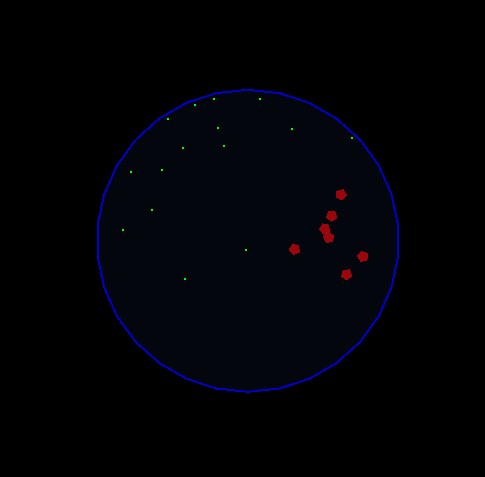
\includegraphics[width=\textwidth]{figures/IMG_ch7/Bursting/RS/RS1} % Adjust the image path as necessary
        \caption{}
        \label{fig:figure1}
    \end{subfigure}
    \hspace{\fill} % Optional: adds space between figures
    \begin{subfigure}{0.48\textwidth}
        \centering
        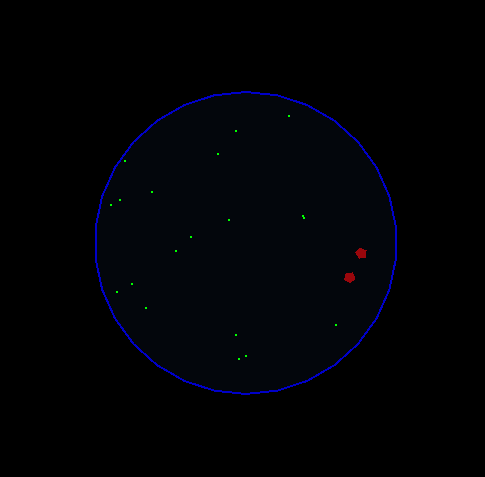
\includegraphics[width=\textwidth]{figures/IMG_ch7/Bursting/RS/RS2} % Adjust the image path as necessary
        \caption{}
        \label{fig:figure2}
    \end{subfigure}


    \caption{(a), Intracellular granules are represented in red, pathogenic particles in green. In this simulation,  when one of each contacts, they anniahilate. (b), the pathogen has replicated and appears to be overcoming the immune challenge of the granules. }
    \label{fig:four_figures}
\end{figure}


\subsection{Model definition}


Both macrophages and neutrophils contain small a number of small packets called granules. These contain oxidative chemicals and are used to kill engulfed pathogen. Neutrophils are of the category ``granulocyte'' and as the name suggests contain a larger number of these packets than macrophages. 

When a count of pathogenic units enters a macrophage by phagocytosis, they begin to face the the action of these granules. Given the packets are finite in number and depletable, it might be that a larger incident cohort of replicators has a greater chance of eventual survival. 

Here we explore a simple model which represents the interplay between the two opposing forces. Replicative pathogenic particles fighting for survival against its host cell's inbuilt defence mechanism. The model thus constitutes two unit types: $\xt$ represents the infectious agents, $\yt$ refers to the remaining number of within-cell granules. From a defined initial condition ($\xx_0, \yy_0$), the dynamic between these two factors results in either pathogen extinction, or the overthrowing of immunity resulting in unbounded growth in $\xt$. Of course, in reality growth will not be truly without limit. Intracellular capacity will eventually introduce a threshold to further expansion without cell bursting.\par
Dynamic transitions are defined quite simple. Units of $\xt$ will divide and increase according to the standard mechanism seen in a birth process. 
$$\pr{\Delta \xt = 1, \Delta \yt = 0} = \lambda \xt \Delta t + o(\Delta t) $$
Suppressive interactions occur with a rate proportional to the product of the two counts, and result in a single elimination of each type.  
 $$\pr{\Delta \xt = -1, \Delta \yt = -1} = \alpha \xt \yt  \Delta t + o(\Delta t) $$
 Hence, with just the addition of a no-event possibility, 
 $$\pr{\Delta \xt = 0, \Delta \yt = 0} = 1 -  \lrb{ \lambda\xt   + \alpha \xt \yt } \Delta t + o(\Delta t) $$
 the continuous time Markov chain is fully defined over infinitesimal durations.


Our focus of interest is in understanding the relationship between incident pathogen count and infection survivability. In other words the probability 
$$\pr{\text{infection survival}} =  1 - \lim_{t\to\infty} \pr{\xt = 0},$$
signifying late time non-extinction. Cases where survival ultimately persists will include the complete exhaustion of antagonistic granules ($\yt = 0$). One may devise a model in which the granules are produced at some rate by the cell, but for now we will aim to understand this more simple version where an initial immune capacity is fixed ($\yy_0$) and never supplemented.  



\subsection{Mathematical definition}


CT Markov process,
$$\mathcal{X} = \{ (\xt, \yt): t\geq 0\},$$
 state space.

$$\mathcal{S} = \{    (i,j)\;\; |\;\; i \in \mathbb{N} \cup \{0\}  ,\;\;j\in\{0,\dots,N\}\} .$$



\begin{figure}[H]\label{grid}
\begin{center}
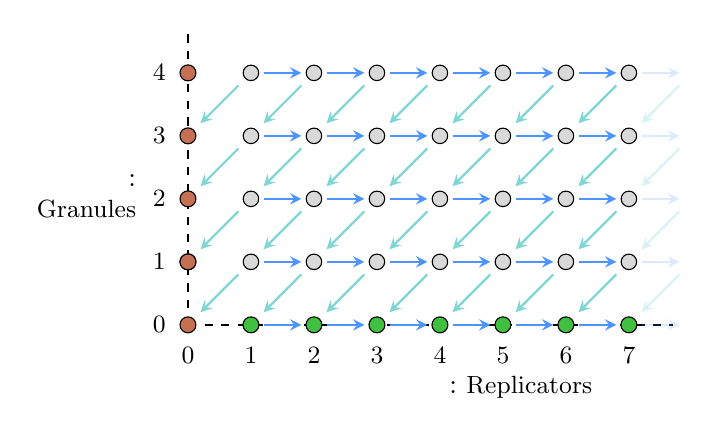
\begin{tikzpicture}[scale=0.8]
% axis and labels 
\draw[thick, dashed] (0,0)--(7.7,0) node[below, yshift=-15pt, xshift=-55pt]{$\xt:$ \small Replicators};
\draw[thick, dashed] (0,0)--(0,4.7) node[left, xshift=-15pt, yshift=-55pt]{$\yt:$} node[left, xshift=-15pt, yshift=-65pt]{\small Granules};
% Grey circles
\foreach \x in {1,2,3,4,5,6,7}
\foreach \y in {1,2,3,4}
\draw[fill = gray1] (\x,\y) circle (3.5pt);
 
 % Axis ticks
\foreach \x in {0,1,2,3,4,5,6,7}
\draw (\x,0) node[below, yshift=-4.5pt]{\small\x} ;
\foreach \y in {0,1,2,3,4}
\draw (0,\y) node[left, xshift=-4.5pt]{\small\y} ;

% Green and red circles
\foreach \x in {1,2,3,4,5,6,7}
\draw[fill = Rec2] (\x, 0) circle (3.6pt);

\foreach \y in {0,1,2,3,4,}
\draw[fill = Rup2] (0, \y) circle (3.6pt);

% Bold transitions diagonal
\foreach \x in {0,1,2,3,4,5,6}
\foreach \y in {1,2,3,4}
{\draw[thick, ->, mut1, >=stealth] (\x+0.8, \y-0.2) -- (\x + 0.2, \y-0.8);}

% Bold horizontal transitions 
\foreach \x in {1,2,3,4,5,6}
\foreach \y in {0,1,2,3,4}
{\draw[>=stealth, ->,thick, na1] (\x+0.2, \y) -- (\x+0.8, \y);}

% Opacity transitions
\foreach \x in {7}
\foreach \y in {0,1,2,3,4}
{\draw[>=stealth, ->,thick, na1, opacity = 0.2] (\x+0.2, \y) -- (\x+0.8, \y);}

\foreach \y in {1,2,3,4}
{\draw[>=stealth, ->,thick, mut1, opacity = 0.3] (7+0.8, \y-0.2) -- (7 + 0.2, \y-0.8);}


\end{tikzpicture}
\end{center}
\caption{State space $\mathcal{S}$ with Ruptured state $R$ in red on the right; green recovery state is seen at (0,0). Arrows show possible transitions between states: \textbf{\textcolor{na1}{blue}} for births and deaths of bacteria type $a$, those of type $b$ are represented by \textbf{\textcolor{nb1}{orange}}, \textbf{\textcolor{mut1}{cyan}} for differentiations from type $a$ to $b$, and \textbf{\textcolor{Rup2}{red}} for the macrophage rupture event.}
\label{grid}
\end{figure}



\begin{figure}[H]\label{grid}
\begin{center}
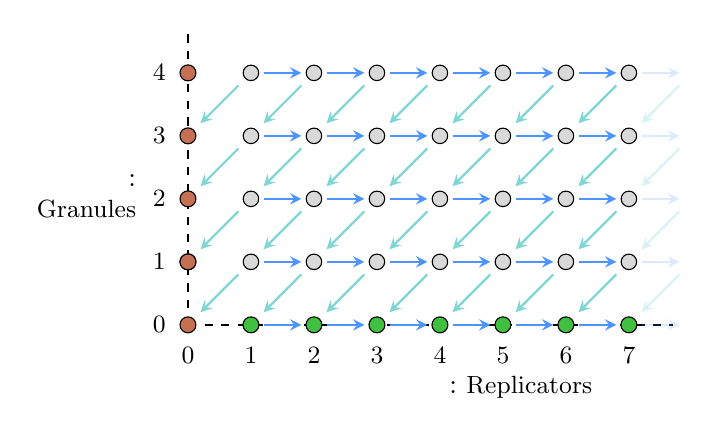
\begin{tikzpicture}[scale=0.8]
% axis and labels 
\draw[thick, dashed] (0,0)--(7.7,0) node[below, yshift=-15pt, xshift=-55pt]{$\xt:$ \small Replicators};
\draw[thick, dashed] (0,0)--(0,4.7) node[left, xshift=-15pt, yshift=-55pt]{$\yt:$} node[left, xshift=-15pt, yshift=-65pt]{\small Granules};
% Grey circles
\foreach \x in {1,2,3,4,5,6,7}
\foreach \y in {1,2,3,4}
\draw[fill = gray1] (\x,\y) circle (3.5pt);
 
 % Axis ticks
\foreach \x in {0,1,2,3,4,5,6,7}
\draw (\x,0) node[below, yshift=-4.5pt]{\small\x} ;
\foreach \y in {0,1,2,3,4}
\draw (0,\y) node[left, xshift=-4.5pt]{\small\y} ;

% Green and red circles
\foreach \x in {1,2,3,4,5,6,7}
\draw[fill = Rec2] (\x, 0) circle (3.6pt);

\foreach \y in {0,1,2,3,4,}
\draw[fill = Rup2] (0, \y) circle (3.6pt);

% Bold transitions diagonal
\foreach \x in {0,1,2,3,4,5,6}
\foreach \y in {1,2,3,4}
{\draw[thick, ->, mut1, >=stealth] (\x+0.8, \y-0.2) -- (\x + 0.2, \y-0.8);}

% Bold horizontal transitions 
\foreach \x in {1,2,3,4,5,6}
\foreach \y in {0,1,2,3,4}
{\draw[>=stealth, ->,thick, na1] (\x+0.2, \y) -- (\x+0.8, \y);}

% Opacity transitions
\foreach \x in {7}
\foreach \y in {0,1,2,3,4}
{\draw[>=stealth, ->,thick, na1, opacity = 0.2] (\x+0.2, \y) -- (\x+0.8, \y);}

\foreach \y in {1,2,3,4}
{\draw[>=stealth, ->,thick, mut1, opacity = 0.3] (7+0.8, \y-0.2) -- (7 + 0.2, \y-0.8);}


\end{tikzpicture}
\end{center}

\label{grid}
\end{figure}


\vspace{5pt}
\noindent



\begin{figure}[H]\label{grid}
\begin{center}
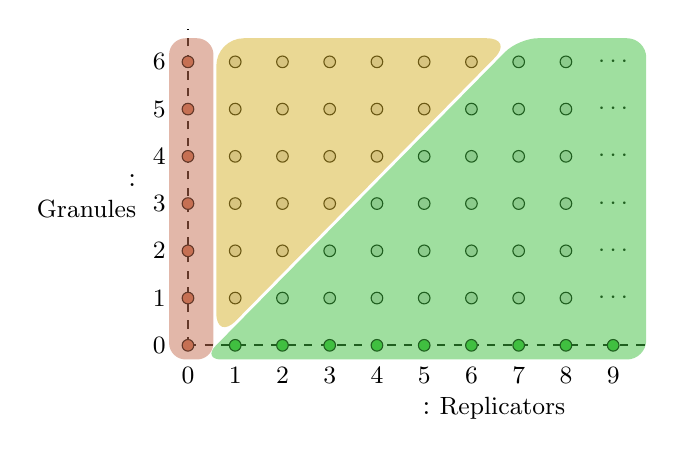
\begin{tikzpicture}[scale=0.6]
% axis and labels 
\draw[thick, dashed] (0,0)--(9.7,0) node[below, yshift=-15pt, xshift=-55pt]{$\xt:$ \small Replicators};
\draw[thick, dashed] (0,0)--(0,6.7) node[left, xshift=-15pt, yshift=-55pt]{$\yt:$} node[left, xshift=-15pt, yshift=-65pt]{\small Granules};
% Grey circles
\foreach \x in {1,2,3,4,5,6,7,8}
\foreach \y in {1,2,3,4,5,6}
\draw[fill = gray1] (\x,\y) circle (3.5pt);

% Grey circles
\foreach \x in {9}
\foreach \y in {1,2,3,4,5,6}
\draw  (\x,\y)node[]{\small$\cdots$};
 
 
 % Axis ticks
\foreach \x in {0,1,2,3,4,5,6,7,8,9}
\draw (\x,0) node[below, yshift=-4.5pt]{\small\x} ;
\foreach \y in {0,1,2,3,4,5,6}
\draw (0,\y) node[left, xshift=-4.5pt]{\small\y} ;

% Green and red circles
\foreach \x in {1,2,3,4,5,6,7,8,9}
\draw[fill = Rec2] (\x, 0) circle (3.5pt);

\foreach \y in {0,1,2,3,4,5,6}
\draw[fill = Rup2] (0, \y) circle (3.5pt);

% Shaded triangle with rounded corners
\fill[fill=nb1, rounded corners=10pt, opacity = 0.5] 
(0.6,6.5) -- (6.9,6.5) -- (0.6,0.1) -- cycle;


\fill[fill=Rec2, rounded corners=7pt, opacity = 0.5] 
(0.3,-0.3) -- (7,6.5) -- (9.7,6.5) -- (9.7, -0.3) -- cycle;

\fill[fill=Rup2, rounded corners=6pt, opacity = 0.5] 
(0.54,-0.3) -- (-0.4,-0.3) -- (-0.4,6.5) -- (0.54,6.5) -- cycle;


\end{tikzpicture}
\end{center}

\label{grid}
\end{figure}



\begin{figure}[H]\label{grid}
\begin{center}
\begin{tikzpicture}[scale=0.7]
% axis and labels 
\draw[thick, dashed] (0,0)--(8.2,0) node[below, yshift=-15pt, xshift=-55pt]{$\xt:$ \small Replicators};
\draw[thick, dashed] (0,0)--(0,6.7) node[left, xshift=-15pt, yshift=-55pt]{$\yt:$} node[left, xshift=-15pt, yshift=-65pt]{\small Granules};
% Grey circles
\foreach \x in {1,2,3,4,5,6,7}
\foreach \y in {1,2,3,4,5,6}
\draw[fill = gray1] (\x,\y) circle (3.5pt);

% Grey circles
\foreach \x in {8}
\foreach \y in {1,2,3,4,5,6}
\draw  (\x,\y)node[]{\small$\cdots$};
 
 % Axis ticks
\foreach \x in {0,1,2,3,4,5,6,7}
\draw (\x,0) node[below, yshift=-4.5pt]{\small\x} ;
\foreach \y in {0,1,2,3,4,5,6}
\draw (0,\y) node[left, xshift=-4.5pt]{\small\y} ;

% Green and red circles
\foreach \x in {1,2,3,4,5,6,7}
\draw[fill = Rec2] (\x, 0) circle (3.5pt);

\foreach \y in {0,1,2,3,4,5,6}
\draw[fill = Rup2] (0, \y) circle (3.5pt);


\filldraw[blue,rounded corners = 1mm, opacity = 0.2]
let \p1=($(1,1)!-2mm!(6,6)$),
\p2=($(6,6)!-2mm!(0,0)$),
\p3=($(\p1)!2mm!90:(\p2)$),
\p4=($(\p1)!2mm!-90:(\p2)$),
\p5=($(\p2)!2mm!90:(\p1)$),
\p6=($(\p2)!2mm!-90:(\p1)$)
in
(\p3) -- (\p4)-- (\p5) -- (\p6) -- cycle;

\filldraw[blue,rounded corners = 1mm, opacity = 0.2]
let \p1=($(1,2)!-2mm!(5,6)$),
\p2=($(5,6)!-2mm!(0,1)$),
\p3=($(\p1)!2mm!90:(\p2)$),
\p4=($(\p1)!2mm!-90:(\p2)$),
\p5=($(\p2)!2mm!90:(\p1)$),
\p6=($(\p2)!2mm!-90:(\p1)$)
in
(\p3) -- (\p4)-- (\p5) -- (\p6) -- cycle;

\filldraw[blue,rounded corners = 1mm, opacity = 0.2]
let \p1=($(1,3)!-2mm!(4,6)$),
\p2=($(4,6)!-2mm!(0,2)$),
\p3=($(\p1)!2mm!90:(\p2)$),
\p4=($(\p1)!2mm!-90:(\p2)$),
\p5=($(\p2)!2mm!90:(\p1)$),
\p6=($(\p2)!2mm!-90:(\p1)$)
in
(\p3) -- (\p4)-- (\p5) -- (\p6) -- cycle;

\filldraw[blue,rounded corners = 1mm, opacity = 0.2]
let \p1=($(1,4)!-2mm!(3,6)$),
\p2=($(3,6)!-2mm!(0,3)$),
\p3=($(\p1)!2mm!90:(\p2)$),
\p4=($(\p1)!2mm!-90:(\p2)$),
\p5=($(\p2)!2mm!90:(\p1)$),
\p6=($(\p2)!2mm!-90:(\p1)$)
in
(\p3) -- (\p4)-- (\p5) -- (\p6) -- cycle;

\filldraw[blue,rounded corners = 1mm, opacity = 0.2]
let \p1=($(1,5)!-2mm!(2,6)$),
\p2=($(2,6)!-2mm!(0,4)$),
\p3=($(\p1)!2mm!90:(\p2)$),
\p4=($(\p1)!2mm!-90:(\p2)$),
\p5=($(\p2)!2mm!90:(\p1)$),
\p6=($(\p2)!2mm!-90:(\p1)$)
in
(\p3) -- (\p4)-- (\p5) -- (\p6) -- cycle;

\filldraw[blue,rounded corners = 1mm, opacity = 0.2]
let \p1=($(1,6)!-2mm!(1,6)$),
\p2=($(1,6)!-2mm!(1,1)$),
\p3=($(\p1)!2mm!90:(\p2)$),
\p4=($(\p1)!2mm!-90:(\p2)$),
\p5=($(\p2)!2mm!90:(\p1)$),
\p6=($(\p2)!2mm!-90:(\p1)$)
in
(\p3) -- (\p4)-- (\p5) -- (\p6) -- cycle;

    % Place text along the line
    \path (1,1) -- (2,2) node[midway, above, sloped, yshift = -5pt] {\tiny  \textbf{\textcolor{blu}{level 1}} };
    \path (1,2) -- (2,3) node[midway, above, sloped, yshift = -5pt] {\tiny  \textbf{\textcolor{blu}{level 2}} };
    \path (1,3) -- (2,4) node[midway, above, sloped, yshift = -5pt] {\tiny  \textbf{\textcolor{blu}{level 3}} };
    \path (1,4) -- (2,5) node[midway, above, sloped, yshift = -5pt] {\tiny  \textbf{\textcolor{blu}{level 4}} };
    \path (1,5) -- (2,6) node[midway, above, sloped, yshift = -5pt] {\tiny  \textbf{\textcolor{blu}{level 5}} };



\end{tikzpicture}
\end{center}

\label{grid}
\end{figure}



\noindent
We can define the process by its 1 step transition probabilities,
$$p_{(i,j)\to\underbar x}(\Delta t) = \pr{\xdt = \underbar x | \xt = (i,j) },$$
for states $(n_a,n_b),x \in \mathcal{S}$. Considering each of the various steps that can be taken from an arbitrary state ($n_a, n_b$) these are as follows.
\begin{equation*}
p_{(i, j)\to\underbar x}(\Delta t) =
\begin{cases}
\alpha_i\Delta t + o(\Delta t)& \underbar x = (i+1,j)\\
\beta_{i,j}\Delta t + o(\Delta t)& \underbar x = (i-1,j-1)\\
1 - (\alpha_i + \beta_{i,j}) \Delta t + o(\Delta t)& \underbar x = (i,j)
\end{cases}
\end{equation*}
(for $\Delta t \rightarrow 0$).


probability of fixation in set ($\xt = 0$, $\yt$) 
$$\theta_{i,j}$$


$$\theta_{i, j} = \hat \alpha_{i,j} \cdot\theta_{i + 1, j} +  \hat \beta_{i,j}  \cdot\theta_{i - 1, j - 1} $$


$$ \hat \alpha_{i,j} = \frac{ \alpha_i }{\alpha_i + \beta_{i,j}} $$
$$ \hat \beta_{i,j} = \frac{ \beta_{i,j} }{\alpha_i + \beta_{i,j}} $$



 first step analysis matrix equation, $\mathbf{p}^{(0)} = \mathbf{A} \cdot \mathbf{p}^{(0)} + \mathbf{c}$


$$
\scriptsize
\begingroup
\renewcommand*{\arraystretch}{1.45}
\begin{bmatrix}
\theta_{1, 1} \\
\theta_{2,2} \\
\theta_{3,3} \\
\theta_{4,4} \\
\theta_{5,5} \\
\theta_{1,2} \\
\theta_{2,3} \\
\theta_{3,4} \\
\theta_{4,5} \\
\theta_{1,3} \\
\theta_{2,4} \\
\theta_{3,5} \\
\theta_{1,4} \\
\theta_{2,5} \\
\theta_{1,5} 
\end{bmatrix}
\endgroup
=
\left[
\renewcommand*{\arraystretch}{1.45} % Adjust this number to increase or decrease row spacing
\begin{array}{ccccc|cccc|ccc|cc|c}
0 & 0 & 0 & 0 & 0 &   0 & 0 & 0 & 0 &   0 & 0 & 0 &   0 & 0 &   0 \vphantom{\frac{1}{2}}\\
\hat \beta_{2,2} & 0 & 0 & 0 & 0 &   0 & 0 & 0 & 0 &   0 & 0 & 0 &   0 & 0 &   0\vphantom{\frac{1}{2}}\\
0 & \hat \beta_{3,3}  & 0 & 0 & 0 &   0 & 0 & 0 & 0 &   0 & 0 & 0 &   0 & 0 &   0\\
0 & 0 & \hat \beta_{4,4}  & 0 & 0 &   0 & 0 & 0 & 0 &   0 & 0 & 0 &   0 & 0 &   0\\
0 & 0 & 0 & \hat \beta_{5,5}  & 0 &   0 & 0 & 0 & 0 &   0 & 0 & 0 &   0 & 0 &   0\\
\hline
0 & \hat\alpha_{1,2} & 0 & 0 & 0 &   0 & 0 & 0 & 0 &   0 & 0 & 0 &   0 & 0 &   0\\
0 & 0 & \hat\alpha_{2,3} & 0 & 0 &   \hat \beta_{2,3}  & 0 & 0 & 0 &   0 & 0 & 0 &   0 & 0 &   0\\
0 & 0 & 0 & \hat\alpha_{3,4} & 0 &   0 & \hat \beta_{3,4}  & 0 & 0 &   0 & 0 & 0 &   0 & 0 &   0\\
0 & 0 & 0 & 0 & \hat\alpha_{4,5} &   0 & 0 & \hat \beta_{4,5}  & 0 &   0 & 0 & 0 &   0 & 0 &   0\\
\hline
0 & 0 & 0 & 0 & 0 &   0 & \hat\alpha_{1,3} & 0 & 0 &   0 & 0 & 0 &   0 & 0 &   0\\
0 & 0 & 0 & 0 & 0 &   0 & 0 & \hat\alpha_{2,4} & 0 &   \hat \beta_{2,4}  & 0 & 0 &   0 & 0 &   0\\
0 & 0 & 0 & 0 & 0 &   0 & 0 & 0 & \hat\alpha_{3,5} &   0 & \hat \beta_{3,5}  & 0 &   0 & 0 &   0\\
\hline
0 & 0 & 0 & 0 & 0 &   0 & 0 & 0 & 0 &   0 & \hat\alpha_{1,4} & 0 &   0 & 0 &   0\\
0 & 0 & 0 & 0 & 0 &   0 & 0 & 0 & 0 &   0 & 0 & \hat\alpha_{2,5} &   \hat \beta_{2,5}  & 0 &   0\\
\hline
0 & 0 & 0 & 0 & 0 &   0 & 0 & 0 & 0 &   0 & 0 & 0 &   0 & \hat\alpha_{1,5} &   0\\

\end{array}
\right]
\begingroup
\renewcommand*{\arraystretch}{1.45}
\begin{bmatrix}
\theta_{1, 1} \\
\theta_{2,2} \\
\theta_{3,3} \\
\theta_{4,4} \\
\theta_{5,5} \\
\theta_{1,2} \\
\theta_{2,3} \\
\theta_{3,4} \\
\theta_{4,5} \\
\theta_{1,3} \\
\theta_{2,4} \\
\theta_{3,5} \\
\theta_{1,4} \\
\theta_{2,5} \\
\theta_{1,5} 
\end{bmatrix}
\endgroup
+
\begingroup
\renewcommand*{\arraystretch}{1.45}
\begin{bmatrix}
\hat \beta_{1,1} \\
0 \\
0 \\
0 \\
0 \\
\hat \beta_{1,2} \\
0 \\
0 \\
0 \\
\hat \beta_{1,3} \\
0 \\
0 \\
\hat \beta_{1,4} \\
0 \\
\hat \beta_{1,5} \\
\end{bmatrix}.
\endgroup
$$



\begin{figure}[H]
    \centering
    \begin{minipage}{0.3\textwidth}
        \centering
        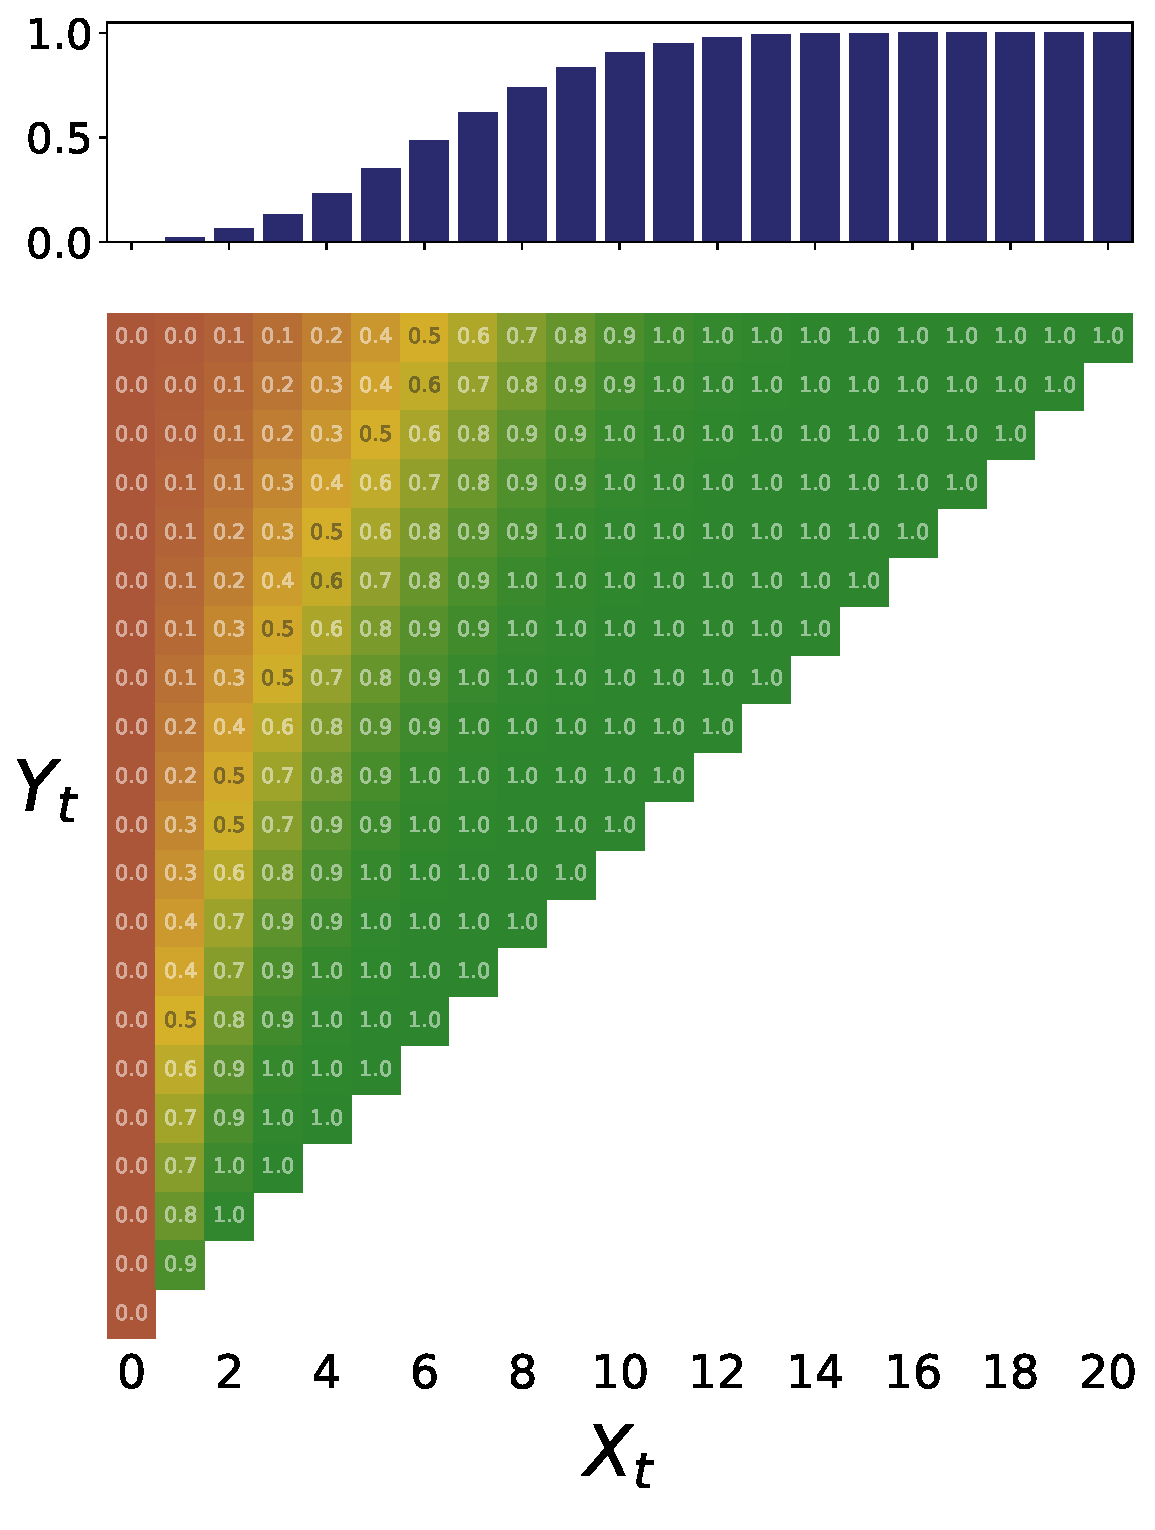
\includegraphics[width=1.1\textwidth]{figures/IMG_ch7/RepSupp_20_0.1_1_NBA_.pdf}
    
        \label{fig:graph1}
    \end{minipage}\hfill
    \begin{minipage}{0.3\textwidth}
        \centering
        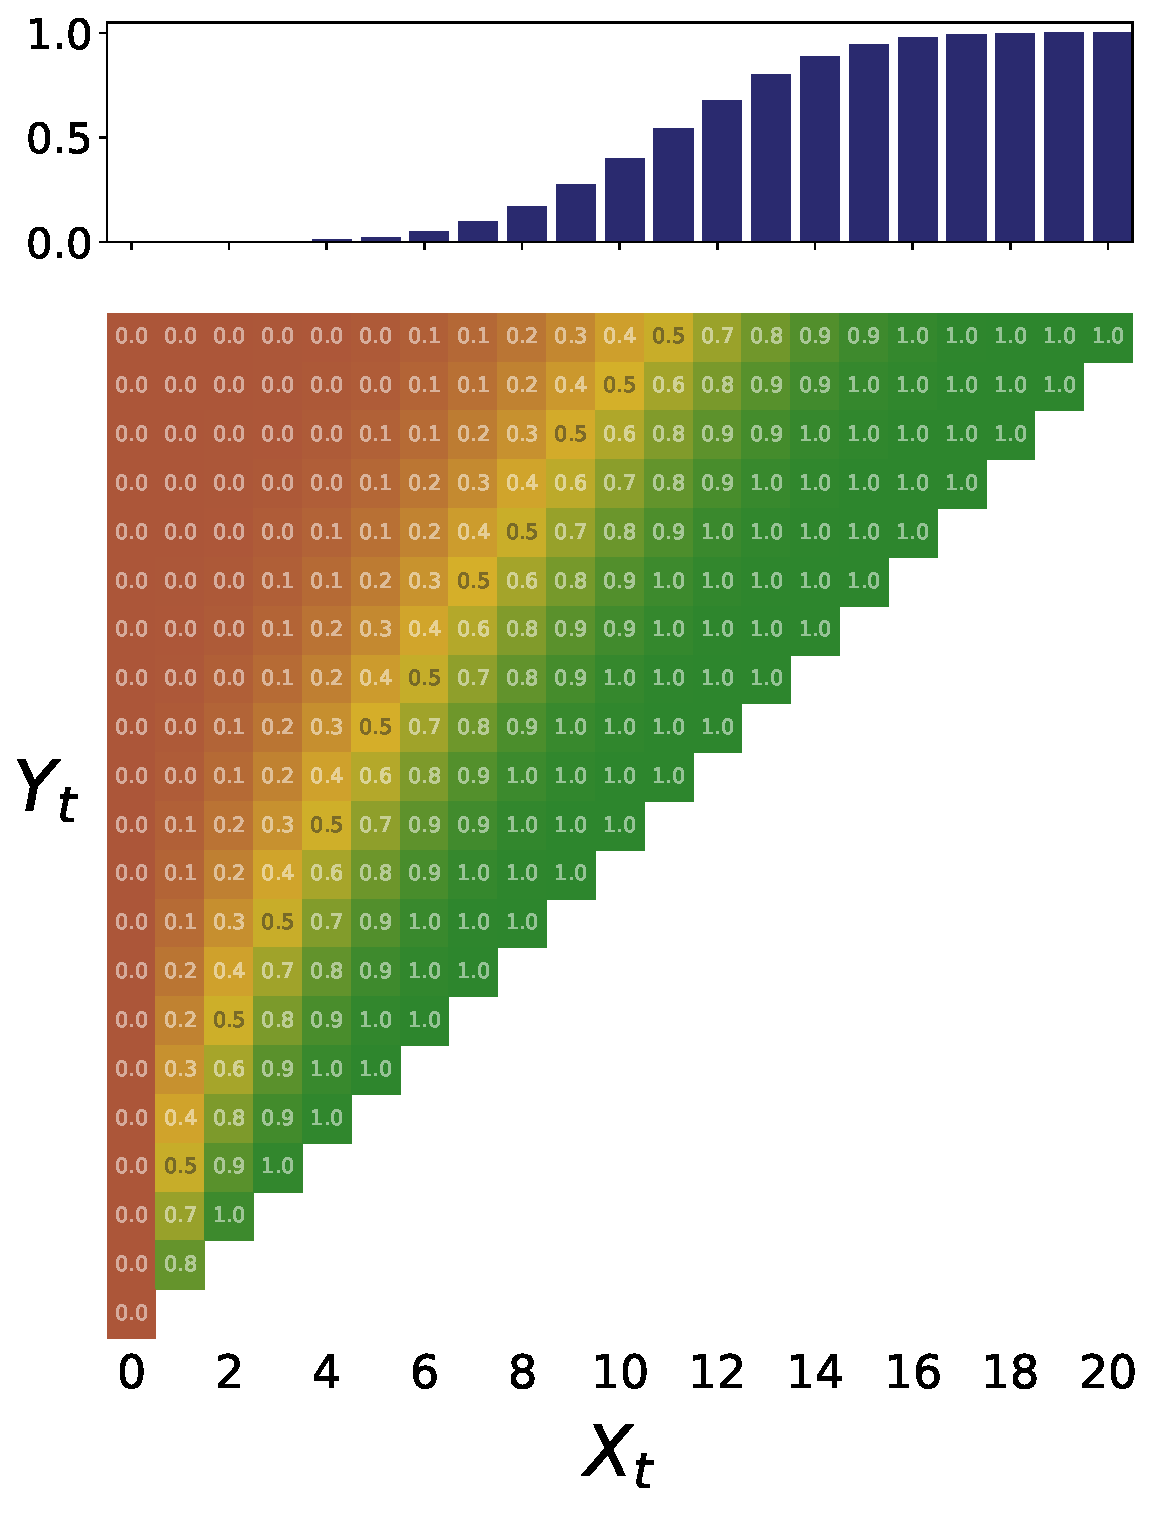
\includegraphics[width=1.1\textwidth]{figures/IMG_ch7/RepSupp_20_0.2_1_NBA_.pdf}
  
        \label{fig:graph2}
    \end{minipage}\hfill
    \begin{minipage}{0.3\textwidth}
        \centering
       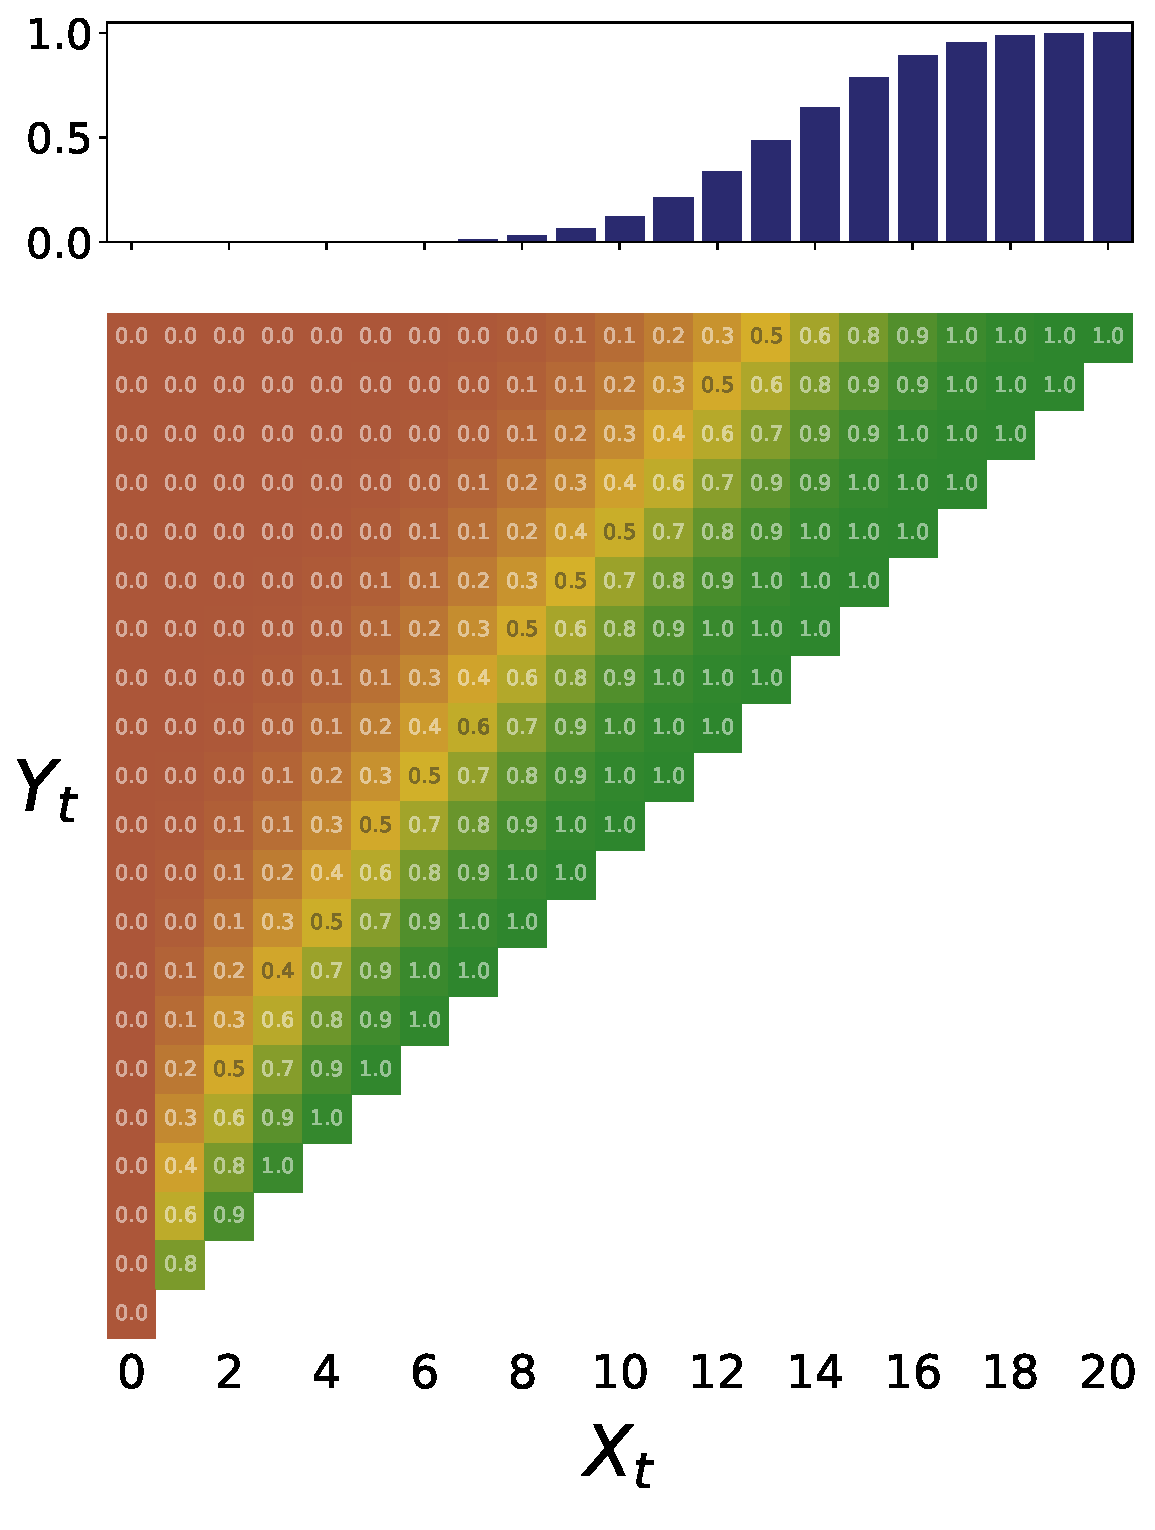
\includegraphics[width=1.1\textwidth]{figures/IMG_ch7/RepSupp_20_0.3_1_NBA_.pdf}
    
        \label{fig:graph3}
    \end{minipage}
    \caption{Probabilities of infection survival given initial count of pathogen ($\xt$), and granules ($\yt$).}
    \label{fig:threegraphs}
\end{figure}



\begin{figure}[h!]
    \centering
    \begin{minipage}{0.3\textwidth}
        \centering
        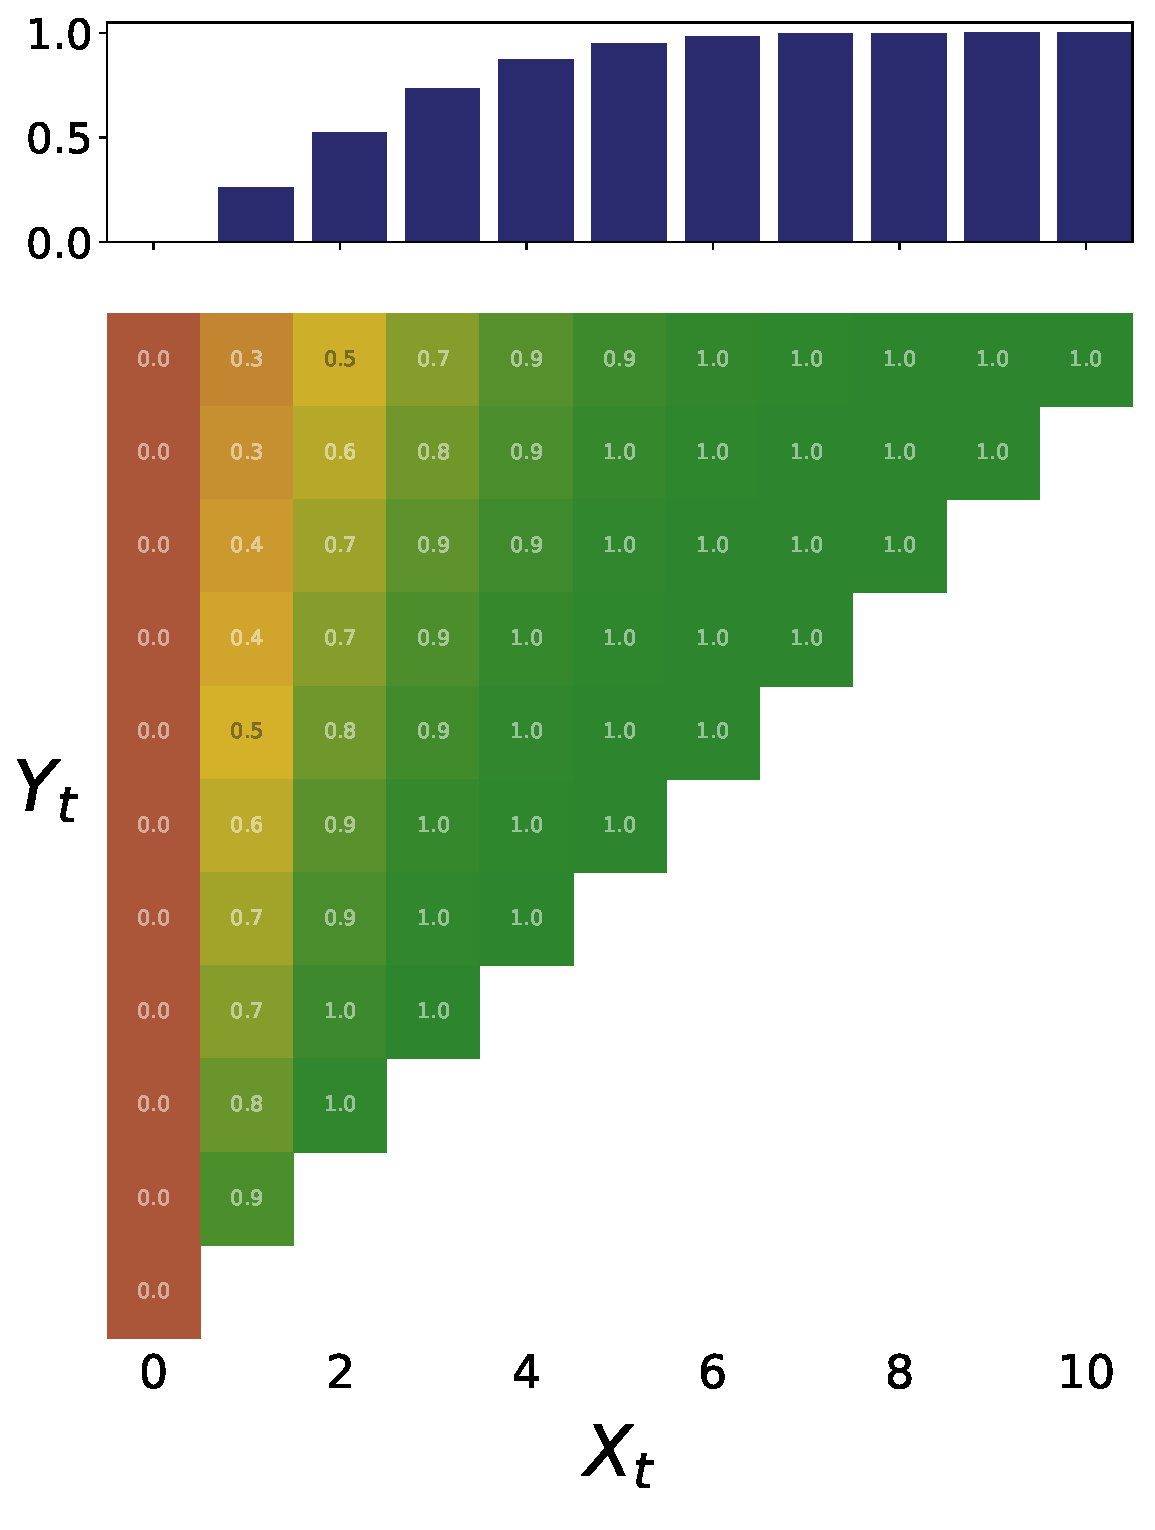
\includegraphics[width=\textwidth]{figures/IMG_ch7/RepSupp_10_0.1_1_NBA_.pdf}
        \label{fig:graph1}
    \end{minipage}\hfill
    \begin{minipage}{0.3\textwidth}
        \centering
        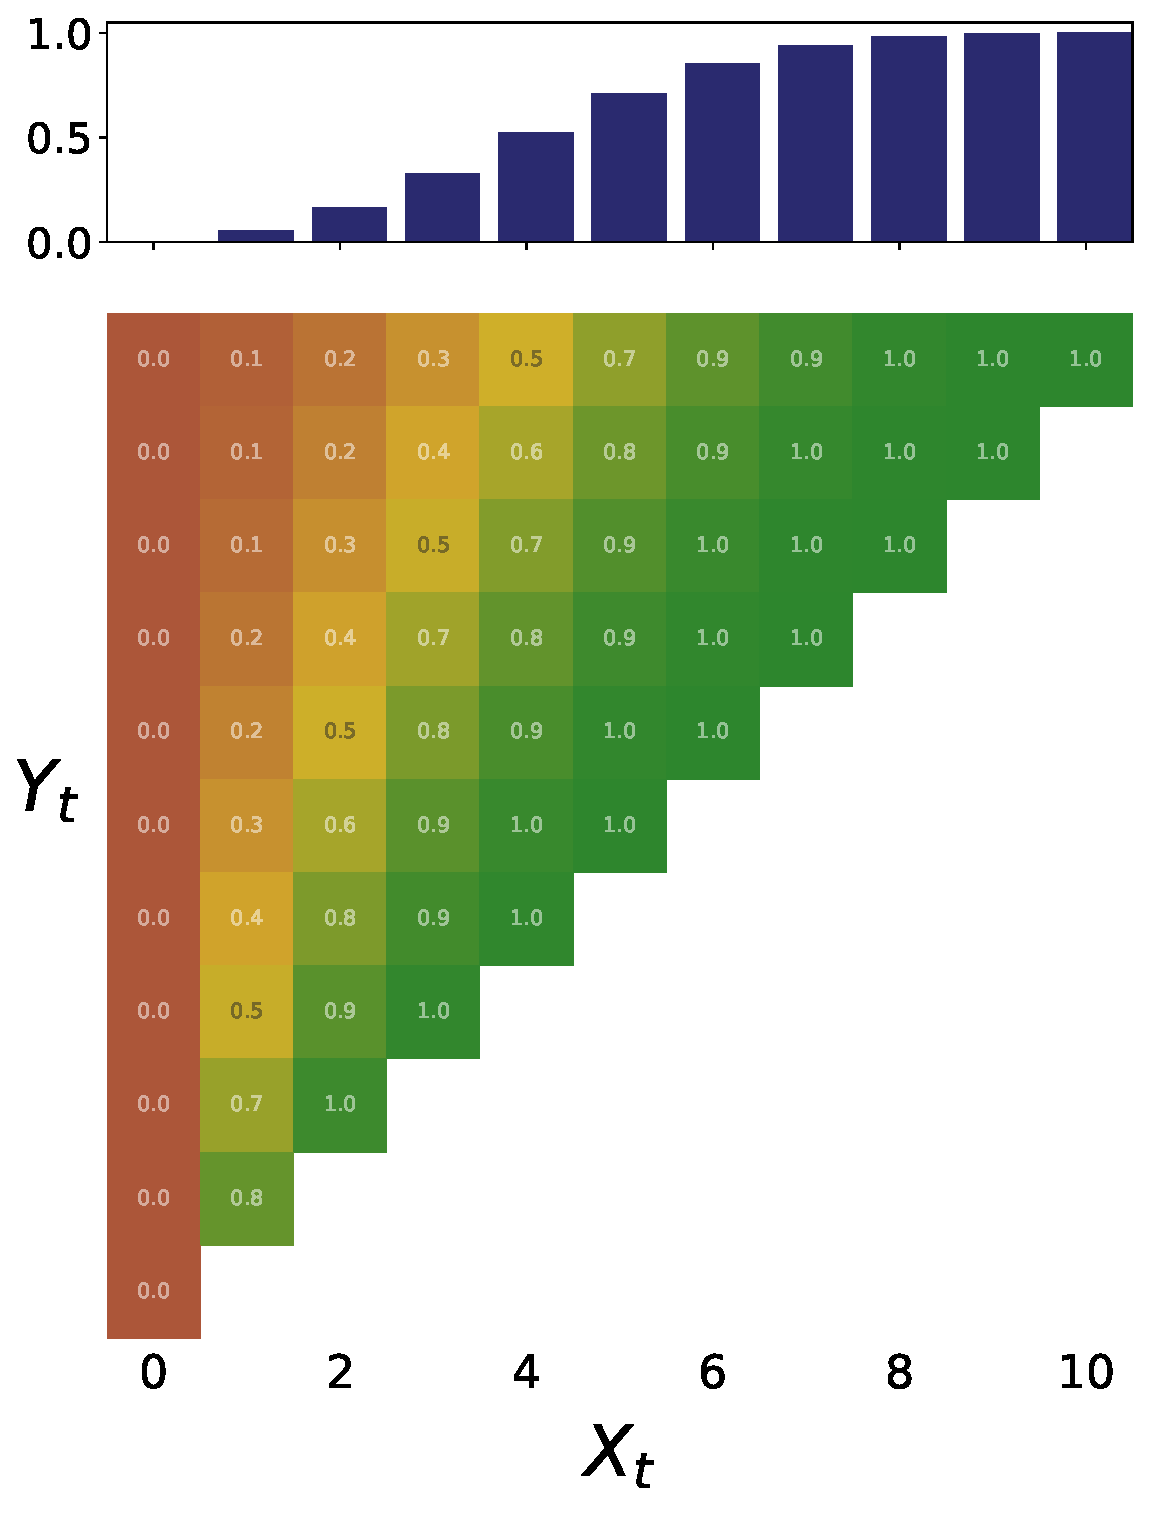
\includegraphics[width=\textwidth]{figures/IMG_ch7/RepSupp_10_0.2_1_NBA_.pdf}
        \label{fig:graph2}
    \end{minipage}\hfill
    \begin{minipage}{0.3\textwidth}
        \centering
       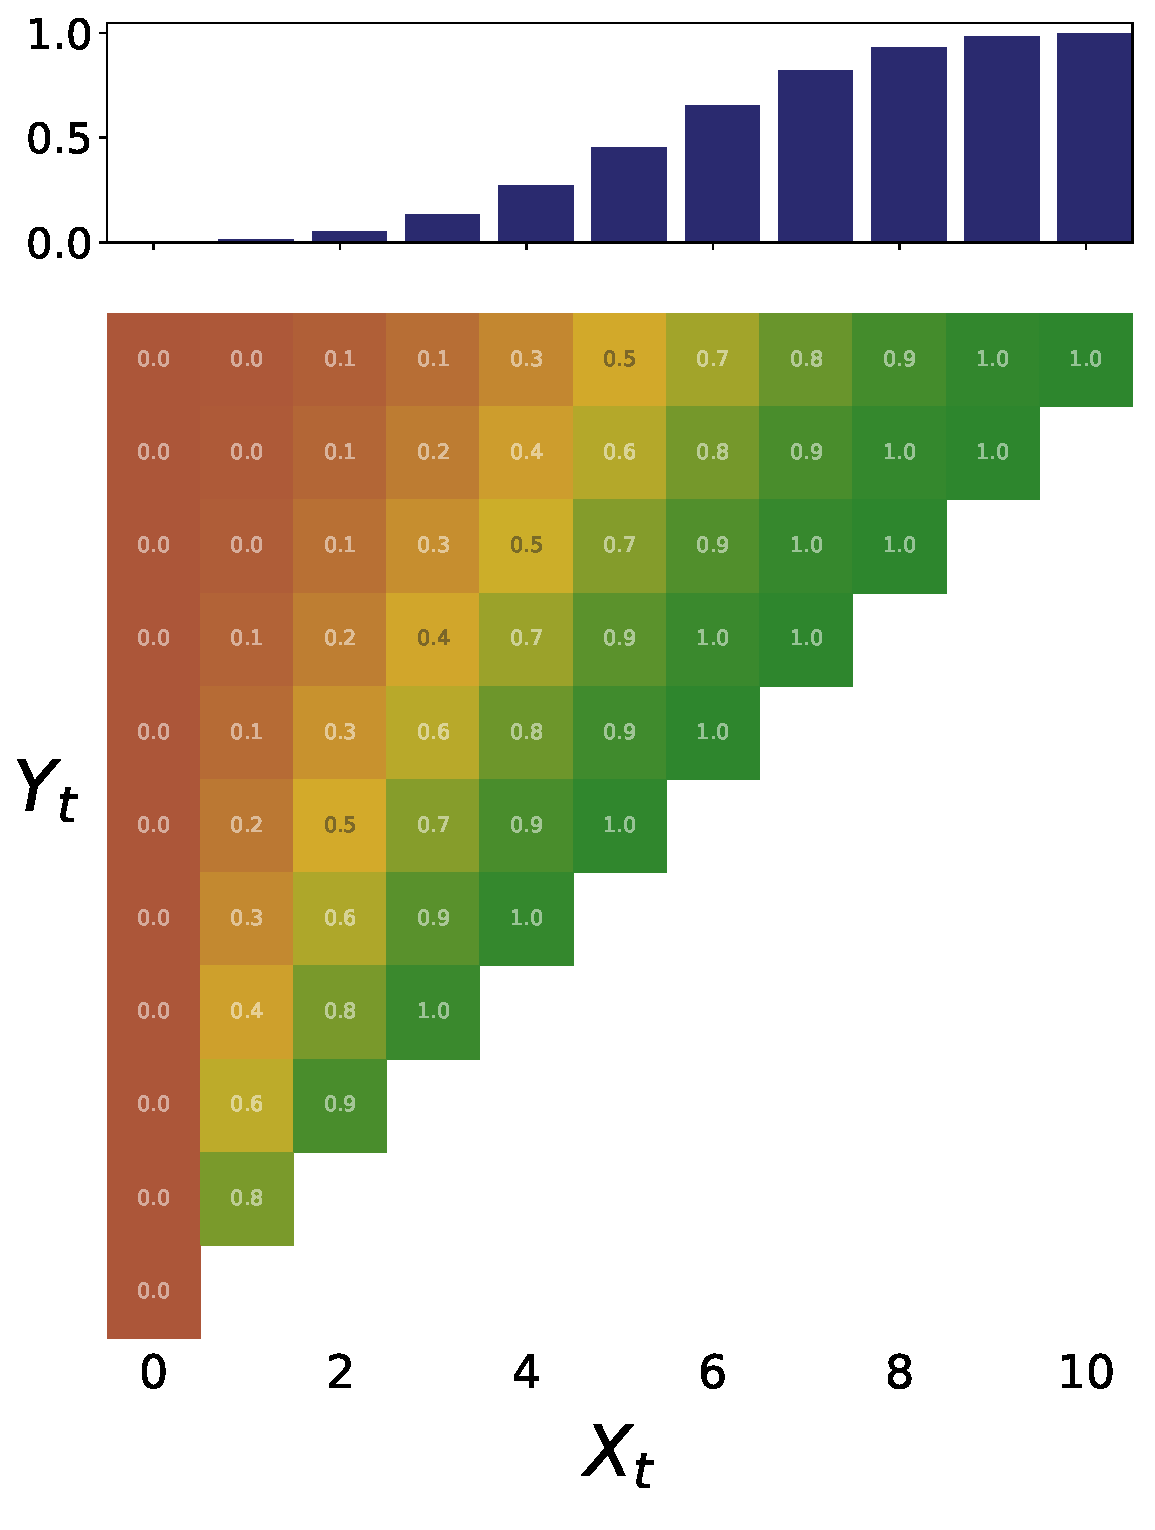
\includegraphics[width=\textwidth]{figures/IMG_ch7/RepSupp_10_0.3_1_NBA_.pdf}
        \label{fig:graph3}
    \end{minipage}
    \caption{For each count of immune granules, there is a critical requirement of incident pathogen for infection persistence to be likely.  This is all to demonstrate that immune granuls create a situation in which bursting dynamics with group transfer could be advantageous. The following section addresses the same sort of dynamics but with regards to extracellular immune factors.}
    \label{fig:threegraphs}
\end{figure}



\begin{lstlisting}[language=Python]
import numpy as np 

N = 20
beta = 0.2
alpha = 1



def b_hat(i, j):
    return (beta * j) / (alpha + beta * j) 

def a_hat(i, j):
    return alpha / (alpha + beta * j)



def generate_Asub(i, j):
    '''produces the A sub-matricies'''
    dim1 = N + 1 - i
    dim2 = N + 1 - j
    Asub = np.zeros((dim1, dim2))
    
    if j - i == 0:
        for k in range(N - j):
            Asub[k+1][k] = b_hat(k+2, k+1+j)
            
        
    if i - j == 1:
        for k in range(N - j):
            Asub[k][k+1] = a_hat(k+1, k+1+j)

    return Asub

def concatA(Amatrix):
    '''combines the A sub-matrices into the full A matrix'''
    w = Amatrix[0].size
    
    # first row
    newA = Amatrix[0][0]
    for j in range(1, w):
        newA = np.append(newA, Amatrix[0][j], axis=1)
    
    # other rows
    for i in range(1,w):
        segmentA = Amatrix[i][0]
        for j in range(1, w):
            segmentA = np.append(segmentA, Amatrix[i][j], axis=1)
        newA = np.append(newA, segmentA, axis=0)
        
    return(newA)

def full_A():
    '''uses above two functions to produce full A matrix'''
    Amat = np.zeros((N, N), dtype=object)
    for i in range(1, N+1):
        for j in range(1, N+1):
            Asub = generate_Asub(i, j)
            Amat[i-1][j-1] = Asub
         
    A_full = concatA(Amat)
    return(A_full)



def generate_Csub(i):
    '''produces the C sub-vectors'''
    dim = N + 1 - i
    Csub = np.zeros(dim)
    Csub[0] = b_hat(1,i)

    return Csub

def concatC(Cvector):
    '''combines the C sub-vectors into the full C vector'''
    newC = Cvector[0]
    for i in range(1, Cvector.size):
        newC = np.append(newC, Cvector[i], axis=0)
    
    return(newC)

def full_C():
    '''uses above two functions to produce full C vector'''
    Cvec = np.zeros(N, dtype = object)
    
    for i in range(1, N+1):
        Csub = generate_Csub(i)
        Cvec[i-1] = Csub 
    
    C_full = concatC(Cvec)
    
    return(C_full[:, np.newaxis])



def get2D_dist(theta_vector):
    '''converts the 1D array with the theta values into its 2D grid form'''
    out = np.zeros((N+1, N+1))
    
    out[0] = np.array([1]*(N+1))
    
    
    idx = 0
    for c in range(N):
        for r in range(N-c):
            i = r+1
            j = r+1+c
        
            out[i][N-j] = round(theta_vector[idx][0], 3)
            
            idx += 1
            
    return out.T



A = full_A()
C = full_C()



# prepares A matrix for linalg solve function 
Amod = np.identity(A.shape[0])-A

# gets theta vector solution 
solution = np.linalg.solve(Amod,C)

# converts to 2D form
dist_2D = get2D_dist(solution)

# switches result from \xt death to survival probability 
dist_2D_survival = np.ones((N+1, N+1)) - dist_2D

# extracts values relevant to initial conditions
ICvec = dist_2D_survival[0]
\end{lstlisting}



%%%%%%%%%%%%%%%%%%%%%%%%%%%%%%%%%%%%%%%%%%%%%%%%%%%%%%%%%%%%%%%%%%%%%%%%%%%%%%%%%%%%%%%%%%%%%%%%%%%%%%%%%%%5
